
%\usepackage[subtle]{savetrees}
%\usepackage[margin=2cm]{geometry}
\usepackage{tikz,amsmath, amssymb,bm,color, amsthm,amsfonts}
\usetikzlibrary{positioning, calc,chains,fit,shapes}
%\usetikzlibrary{circuits.logic.US,circuits.logic.IEC,fit}
\usepackage{enumerate}
\usepackage{comment}
\usepackage{tikz}
\usepackage{graphics}
%\usepackage[cm]{fullpage}
\usepackage{longtable}
\usepackage{mdframed}
\usepackage{caption}
\usepackage{subcaption}
\usepackage{slashbox}
\usepackage{url}
\usepackage{framed}
\usepackage{array}
\usepackage{tabu}
\usepackage{lscape}
\usepackage{multirow}
\usepackage{ulem}
\usepackage{multicol}
\usepackage{placeins}
\usepackage{cite}
\usepackage{enumitem}
\usepackage{mathtools}
%\usepackage[numbers]{natbib}
%\usepackage{mathtools}
%\usepackage{authblk}

\mdfsetup{skipabove=2pt,skipbelow=2pt}
%\setlenght {\marginparwidth }{2cm}
%\usepackage{todonotes}

%\usepackage{floatrow}
%\usepackage{adjustbox}
%\setlength{\extrarowheight}{.05ex}
%\renewcommand\thesubfigure{\roman{subfigure}}


%\newtheorem{theorem}{Theorem}[section]
%\newtheorem{lemma}[theorem]{Lemma}
%\newtheorem{observation}[theorem]{Observation}
%\newtheorem{corollary}[theorem]{Corollary}
%\newtheorem{proposition}[theorem]{Proposition}
%\newtheorem{definition}[theorem]{Definition}
\newtheorem{construction}{Construction}
%\newtheorem{conjecture}{Conjecture}
%\newtheorem{remark}[theorem]{Remark}

\newcommand{\pname}[1]{\textnormal{\textsc{#1}}}
\newcommand{\cclass}[1]{\textnormal{\textsf{#1}}}
\newcommand{\nog}{nine} % no of members in the gang!
\newcommand{\nogd}{nineteen} % no of members in the gang - for deletion/completion
\newcommand{\nogl}{eighteen} % no of members in the larger gang - for editing
\newcommand{\nogld}{thirty eight} % no of members in the larger gang - for deletion/completion
\newcommand{\diffnog}{ten} %
%\newcommand{\dominatedby}{dominated by} %
%\newcommand{\dominatingset}{dominating set} %
%\newcommand{\dominates}{dominates} %
\newcommand{\simulates}{simulates} %
\newcommand{\baseset}{base} %
\newcommand{\issimulatedby}{is simulated by} %

\newcommand{\StarSAT}{\pname{8-SAT$_{\geq 6}$}}
\newcommand{\FSAT}{\pname{4-SAT$_{\geq 2}$}}
\newcommand{\FISAT}{\pname{5-SAT$_{\geq 3}$}}
\newcommand{\SIXSAT}{\pname{6-SAT$_{\geq 4}$}}
\newcommand{\ESAT}{\pname{8-SAT$_{\geq 6}$}}
\newcommand{\KSAT}{\pname{$k$-SAT$_{\geq {k-2}}$}}
\newcommand{\KSATO}{\pname{$k$-SAT}}
\newcommand{\ESATO}{\pname{8-SAT}}
\newcommand{\FSATO}{\pname{4-SAT}}
\newcommand{\FISATO}{\pname{5-SAT}}
\newcommand{\TSAT}{\pname{3-SAT}}
\newcommand{\HED}{\pname{${H}$-free Edge Deletion}}
\newcommand{\AEE}{\pname{${A}$-free Edge Editing}}
\newcommand{\AED}{\pname{${A}$-free Edge Deletion}}
\newcommand{\TSED}{\pname{$t$-star-free Edge Deletion}}
\newcommand{\ATSED}{\pname{Annotated $t$-star-free Edge Deletion}}
\newcommand{\AFSED}{\pname{Annotated $4$-star-free Edge Deletion}}
\newcommand{\FSED}{\pname{$4$-star-free Edge Deletion}}
\newcommand{\FVSED}{\pname{$5$-star-free Edge Deletion}}
\newcommand{\HEE}{\pname{${H}$-free Edge Editing}}
\newcommand{\HEC}{\pname{${H}$-free Edge Completion}}
\newcommand{\HDEE}{\pname{${H'}$-free Edge Editing}}
\newcommand{\HDDEE}{\pname{${H''}$-free Edge Editing}}
\newcommand{\HDED}{\pname{${H'}$-free Edge Deletion}}
\newcommand{\HDEC}{\pname{${H'}$-free Edge Completion}}
\newcommand{\HBEE}{\pname{${\overline{H}}$-free Edge Editing}}
\newcommand{\HBED}{\pname{${\overline{H}}$-free Edge Deletion}}
\newcommand{\HBEC}{\pname{${\overline{H}}$-free Edge Completion}}
\newcommand{\HOEDCE}{\pname{${H_1}$-free Edge Deletion(Completion/Editing)}}
\newcommand{\HEDCE}{\pname{${H}$-free Edge Deletion(Completion/Editing)}}
\newcommand{\HEEDC}{\pname{${H}$-free Edge Editing(Deletion/Completion)}}
\newcommand{\HDEEDC}{\pname{${H'}$-free Edge Editing(Deletion/Completion)}}
\newcommand{\BFED}{\pname{Bow-free Edge Deletion}}
\newcommand{\ABFED}{\pname{Annotated Bow-free Edge Deletion}}
\newcommand{\DTIS}{\pname{Distance-3 Independent Set}}
\newcommand{\SVC}{\pname{Strong Vertex Cover}}
\newcommand{\CLIQUE}{\pname{Clique}}
\newcommand{\IS}{\pname{Independent Set}}
\newcommand{\PFS}{\pname{Propagational-$f$ Satisfiability}}
\newcommand{\RHED}{\pname{Restricted ${H}$-free Edge Deletion}}
\newcommand{\RHEC}{\pname{Restricted ${H}$-free Edge Completion}}
\newcommand{\RHDED}{\pname{Restricted ${H'}$-free Edge Deletion}}
\newcommand{\RHDEC}{\pname{Restricted ${H'}$-free Edge Completion}}
\newcommand{\RHEE}{\pname{Restricted ${H}$-free Edge Editing}}
\newcommand{\PH}{$\cclass{NP} \subseteq \cclass{coNP/poly}$}
\newcommand{\NOPH}{$\cclass{NP} \not\subseteq \cclass{coNP/poly}$}
\newcommand{\LG}{\mathcal{W}}
\newcommand{\LGD}{\mathcal{W}'}
\newcommand{\LGDD}{\mathcal{W}''}


%\let\oldvee\vee
\renewcommand\vee{\boxtimes}

\newcommand\addvmargin[1]{
  \node[fit=(current bounding box),inner ysep=#1,inner xsep=0]{};
}
\setlength{\fboxrule}{0pt}

\newcommand{\defstage}[2]{% PGD Version
  \hfill\\\smallskip\noindent%
  \begin{tabularx}{\textwidth}{|l X|}%
    \hline%
    \multicolumn{2}{|l|}{\textbf{#1}}\\%
    &#2\\\hline%
  \end{tabularx}%
%  \smallskip%
}
\setlength\extrarowheight{15pt}

\newcounter{rowcntr}[table]
\renewcommand{\therowcntr}{\thetable.\arabic{rowcntr}}

% A new columntype to apply automatic stepping
\newcolumntype{N}{>{\refstepcounter{rowcntr}\therowcntr}c}

% Reset the rowcntr counter at each new tabular
\AtBeginEnvironment{longtabu}{\setcounter{rowcntr}{0}}

\newcounter{rowcntra}[table]
\renewcommand{\therowcntra}{\arabic{rowcntra}}

% A new columntype to apply automatic stepping
\newcolumntype{M}{>{\refstepcounter{rowcntra}\therowcntra}c}

% Reset the rowcntr counter at each new tabular
\AtBeginEnvironment{tabular}{\setcounter{rowcntra}{0}}

\newcommand{\NPC}{NP-Complete}


\newcommand{\highlight}[1]{\textcolor{blue}{#1}}
\newcommand{\dhanya}[1]{\textcolor{blue}{dhanya: #1}}


%\newcommand{\XCD1}[1]{\pname{$\chi_{cd}$\ensuremath{(#1)}}}
\newcommand{\XCD}{\pname{$\chi_{cd}$}}
\newcommand{\SC}{\pname{$\omega_{s}$}}

\newcommand{\CDC}{\textsc{CD-coloring}}
\newcommand{\SCP}{\textsc{Separated-Cluster}}
\newcommand{\TD}{\textsc{Total Domination}}
\newcommand{\ISP}{\textsc{Independent Set}}
\newcommand{\CC}{\textsc{Clique Cover}}
\newcommand{\TETHS}{Further, the problem cannot be solved in time \ensuremath{2^{o(|V(G)|)}}, unless the ETH fails}
%\usetikzlibrary{positioning,chains,shapes,calc}
\usetikzlibrary{fit}
\thispagestyle{empty}
\usetikzlibrary{
  graphs,
  graphs.standard
}
\setbeamertemplate{itemize item}{\textbullet}
% Define a boolean parameter
\newboolean{longtalk}
\setboolean{longtalk}{false} % Set to 'true' to show the slides, 'false' to hide them


\newcommand{\takeaways}{
\begin{itemize}
\item Decentralized exchanges are designed for \emph{passive} liquidity provision.
\item Fixed costs to participate in markets lead to different economies of scale for heterogeneous \textbf{LP}s.
\item If fragmented: high-fee pools tend to have lower execution, lower liquidity yields and higher adverse selection cost.
\item But, fragmentation can be efficient.
\end{itemize}

\begin{center}
\begin{tabular}{ll}
\toprule
Low-fee pools & High-fee pools \\
\cmidrule{1-2}
High trading volume & Low trading volume \\
Low aggregate liquidity & High aggregate liquidity \\
Few, large \textbf{LP}s & Many, small \textbf{LP}s \\
Short liquidity cycles & Large liquidity cycles \\
\bottomrule
\end{tabular}
\end{center}

}

\begin{document}



\title{Fragmentation and Optimal Liquidity Supply on Decentralized Exchanges} 
\author[Lehar, Parlour, Zoican]{Alfred Lehar, Christine A. Parlour, and Marius Zoican}

\date{March 2024}

\institute[U Toronto]{Haskayne School of Business, University of Calgary \and Haas School of Business, UC Berkeley \and Rotman School of Management,  University of Toronto}

\begin{frame}[noframenumbering]
\titlepage
\end{frame}

\begin{frame}\frametitle{This paper}
\begin{itemize}
\item Use design of  an automated market maker (AMM) to study:
\medskip
\begin{itemize}
\item[\textbullet] Effect of fixed and variable costs on liquidity supply
\smallskip
\item[\textbullet] Find that fragmented liquidity can be beneficial
\end{itemize}
\bigskip
\item Why study an AMM?
\begin{enumerate}
\item They process a large volume of transactions.
\smallskip
\item They seem to provide more liquidity than centralized limit order markets.
\smallskip
\item As real world assets (RWA) move to tokenization models, trading may migrate.
\smallskip
\item Costs/benefits to supplying liquidity is cleaner to observe than in centralized markets.
\end{enumerate}

\end{itemize}


\end{frame}

\begin{frame}{Decentralized exchanges (DEX) trade}
    \begin{center}
        % Figure removed
    \end{center}
\end{frame}

\begin{frame}{DEX have substantial liquidity (at least in major pairs)}
    \begin{center}
        % Figure removed
    \end{center}
\end{frame}


\begin{frame}\frametitle{Uniswap - Details}
\begin{itemize}
\item UniSwap is a decentralized protocol originally on the Ethereum Blockchain
\item Uniswap comprises tens of thousands of liquidity pools
\begin{itemize}
\item[\textbullet] Each pool has two assets -- all trades are swaps
\end{itemize}
\bigskip
\item There are three versions of Uniswap (v1,v2,v3)
\medskip
\item Features common to all versions:
\begin{itemize}
\item[\textbullet] Agents choose to supply or demand liquidity
\item[\textbullet] Transaction prices are automatically calculated as a function of liquidity demand and supply.
\item[\textbullet] Only payoff for liquidity supplier is a \% fee paid by the liquidity demander.
\end{itemize}
\medskip
\item Unique to v3
\begin{itemize}
\item[\textbullet] Variable fees:  Each asset pair can trade in 1, 5, 30 or 100bps pools.
\item[\textbullet] Concentrated liquidity:  Liquidity suppliers can choose the price range over which they supply liquidity 
\end{itemize}
\end{itemize}
\end{frame}


\begin{frame}\frametitle{Uniswap -- Liquidity Provision v2 \\ A Pool with Ethereum ``E'' and a token ``T''}

\begin{minipage}{0.35\textwidth}%
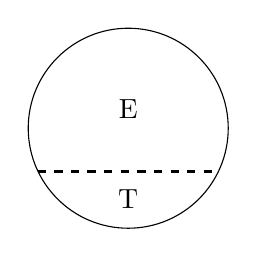
\begin{tikzpicture}
\draw(0,1) circle(0.5in);
\draw[thick,dashed](-1.15,0.45)--(1.15,0.45);
\draw(0,1) node[above]{E};
\draw(0,0.35) node[below]{T};
\end{tikzpicture}
\end{minipage} %
\begin{minipage}{0.55\textwidth}%
\begin{itemize}
\item Liquidity suppliers deposit Eth and T

\medskip
\item Liquidity demander who buys the token, removes it from the pool and deposits Eth.
\item Liquidity demander who sells the token, adds it to the pool and withdraws Eth.

\bigskip
\item Liquidity demanders pay a fixed, proportional fee which is passed through to the liquidity suppliers.

\end{itemize}
\end{minipage}

\end{frame}




\begin{frame}\frametitle{Price Impact to sell $\Delta_T$ tokens}
\begin{minipage}{0.25 \textwidth}
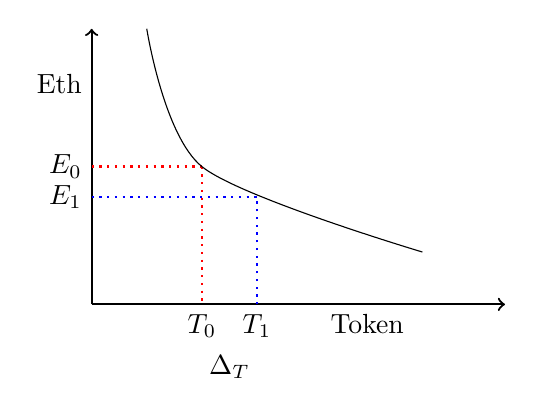
\begin{tikzpicture}[scale=0.35]
\draw[thick,->] (0,0)-- (15,0);
\draw[thick,->] (0,0) -- (0,10);
\draw (0,8) node[left]{Eth};
\draw(10,0) node[below]{Token};
\draw[dotted,red, thick](0,5)--(4,5);
\draw[dotted,red,thick](4,5)--(4,0);
\draw (0,5) node[left]{$E_0$};
\draw (4,0) node[below]{$T_0$};
\draw(6,0) node[below]{$ T_1$};
\draw(5,-1.5) node[below] {$\Delta_T$}; 
\draw[dotted,blue,thick](6,0)--(6,3.9);
\draw[dotted,blue,thick](0,3.9)--(6,3.9);
\draw(0,3.9) node[left]{$E_1$};
\draw plot[smooth] coordinates {(2,10)  (4,5) (12,1.9)};
\end{tikzpicture}
\end{minipage}
\begin{minipage}{0.2\textwidth}
\hspace{1in}
\end{minipage}
\begin{minipage}{0.45 \textwidth}
\begin{itemize}
\item For negligible quantities, the exchange between Eth and the Token is E/T
\item For larger trades, the exchange rate is determined by a ``bonding curve.''
\item For given $E$ and $T$, so $ET=k$: \end{itemize}
\begin{eqnarray*}
(E + \Delta_E)(T+\Delta_T) = k
\end{eqnarray*}
\begin{itemize}
\item As more liquidity is supplied, bonding curve shifts out.
\end{itemize}
\end{minipage}
\end{frame}

\begin{frame}{Unique to v3:  Concentrated Liquidity}
\begin{itemize}
    \item On Uniswap v3, liquidity providers can specify price limits on their positions.
    \item If the current pool price (e.g., ``midpoint'') is outside the range, the position does not earn fees.
    \item $\rightarrow$ incentive to re-price the position to capture fees.
\end{itemize}
    \begin{center}
        % Figure removed
    \end{center}
\end{frame}

\begin{frame}
\frametitle{Managing liquidity on DEX is costly}
\begin{center}
   % Figure removed
\end{center}
\end{frame}

\begin{frame}{Fixed cost of supplying liquidity (gas fee) on Uniswap v3}
    \begin{center}
        % Figure removed
    \end{center}
\end{frame}




\ifthenelse{\boolean{longtalk}}{
\begin{frame}{Liquidity Provision on a DEX}

\bigskip

    \begin{enumerate}
    \item Unique laboratory to study how transaction costs affect the market for liquidity.
        \item DEX  designed for \textbf{passive} liquidity provision. \vspace{0.05in}
        %\item ``\emph{Set-it-and-forget-it}'' liquidity: i.e., what ETFs did for portfolio management. \vspace{0.05in}
        \item On v3 actively managing liquidity is costly:
            \begin{enumerate}
                \item \emph{gas price} from interacting with Ethereum blockchain. \vspace{0.05in}
                \item \emph{time/effort} to monitoring the position.
            \end{enumerate}
        \vspace{0.05in}
        %\item Economies of scale: small liquidity providers face higher relative costs.\vspace{0.05in}
         
    \end{enumerate}
    \medskip

    
    \end{frame} }

% \begin{frame}{Decentralized exchanges $\approx$ 20\% of crypto trading volume}
%     \begin{center}
%         % Figure removed
%     \end{center}
% \end{frame}







\begin{frame}\frametitle{Results}

\vspace{0.1in}

\begin{alertblock}{Theory and  evidence of LP ``clienteles'' based on their scale:}
\bigskip

\begin{enumerate}
    \item Small LPs are more passive, have  lower fill rates but get high fees. 
    \bigskip
    \item Large LPs are more active, have higher fill rates but get low fees.
    \bigskip
    \item This segmentation can be efficient
\end{enumerate}


\end{alertblock}

\end{frame}

%\section{Model}

\begin{frame}{Model}

\begin{block}{Asset and markets.} \begin{itemize}
    \item Token with expected value $v$ trades on two liquidity pools with fees $h>\ell>0$.
    \item Fixed cost $\Gamma>0$ of interacting with the pool (e.g., gas fee).
\end{itemize}
\end{block}

\begin{block}{Liquidity providers (\textbf{LP})}

 \begin{tabular}{cl}  
     \begin{tabular}{l}
            \parbox{0.35\linewidth}{%  change the parbox width as appropriate
                \begin{itemize}
        \item Risk-neutral;
        \item Token endowments $q_i$; \item $q_i$ follows a bounded Pareto distribution:
        \begin{equation*}\label{eq:density}
    \varphi\left(q\right)=\Big(\frac{Q}{Q-1}\Big) \frac{1}{q^2}.
    \end{equation*}
    \end{itemize}}
       \end{tabular}
    &\begin{tabular}{c}
            % Figure removed
        \end{tabular}  
   \end{tabular}

\end{block}

\end{frame}



\begin{frame}{Timeline}

\begin{block}{Liquidity takers (\textbf{LT}).} Two types of $\textbf{LT}$: 
\begin{enumerate}
    \item \emph{small} $\textbf{LT}$ arrive at constant rate $\theta \diff t$ and optimally go to the low-fee pool first ($\ell$). 
    \item \emph{large} $\textbf{LT}$ demand $\Theta$ token units and arrive as Poisson process $J_t\left(\lambda\right)$. \\ They are exogenously large enough to consume all liquidity on $\ell$ and $h$ pools.
\end{enumerate}
\end{block}
\vspace{0.1in}
    \begin{center}
        % Figure removed
    \end{center}


\end{frame}

\begin{frame}\frametitle{Prices}
\begin{itemize}
\item We assume a linear bonding curve -- prices occur at $v$.
\bigskip
\item Traditionally, a spread compensates market makers for adverse selection \\ (``insider trading") \vspace{0.1in}
\item In these markets 
\begin{enumerate}
    \item liquidity providers do not post or earn a spread
    \item as these are assets with no cash flows, unclear what form adverse selection takes
    \item no clear ``value" benchmarks as off chain assets have a different use value. 
\end{enumerate}
\end{itemize}

    
\end{frame}



\begin{frame}{The liquidity provider problem}
\begin{itemize}
\item ${\color{red} d_k}$ is the endogenous liquidity cycle duration, which $\nearrow$ in aggregate liquidity:
\begin{eqnarray*}
d_h & = & \frac{1}{\lambda}\\
    d_\ell&=&\frac{1}{\lambda}-\frac{1}{\lambda}\exp\left(-\frac{\LL}{\theta}\lambda\right) 
\end{eqnarray*}
where $\LL$ is the aggregate liquidity on the low-fee pool.
\medskip
 \item Liquidity providers choose pool $k^\star$ to maximize expected profit per unit of time:
\begin{equation*}
\label{eq:optimal_pool}
    k^\star\left(q_i\right) = \arg\max_{\left\{\ell,h,\emptyset\right\}}   \Big[\frac{q_i \ell - \Gamma}{d_\ell} , \; \frac{q_i h -\Gamma}{d_h}, \; \emptyset\Big].
\end{equation*}
\item Trade-off between:
\begin{enumerate}
   \item higher liquidity fee per unit of time in low fee pools, and 
    \item lower rebalancing cost in high-fee pools.
\end{enumerate}
\end{itemize}
\end{frame}

\begin{frame}{Equilibrium}
\begin{itemize}
\item There is a threshold endowment $\qmg$ such that all $\LP$s with $q_i>\qmg$ post liquidity on the low-fee pool and all $\LP$s with $q_i\leq \qmg$ choose the high-fee pool. 
\begin{align*}\label{eq:liquidity_levels}
    \LL&=\int_{\qmg}^Q q_i \varphi\left(q_i\right) \diff i = \frac{Q}{Q-1}\left(\log Q - \log \qmg \right)  \text{ and }\nonumber \\
    \LH&=\int_{\underline{q}}^{\qmg}  q_i \varphi\left(q_i\right) \diff i = \frac{Q}{Q-1}\left(\log \qmg - \log \underline{q}\right)
\end{align*}
\end{itemize}
\bigskip
\begin{center}
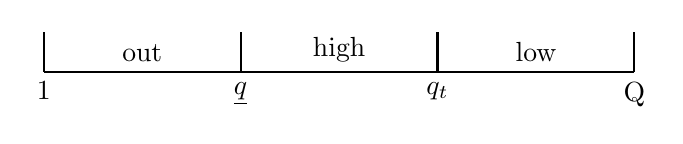
\begin{tikzpicture}[scale= 0.5]
    \draw[thick] (0,0)--(15,0);
    \draw[thick] (10,0)--(10,1);
    \draw[thick] (15,0)--(15,1);
    \draw[thick] (0,0)--(0,1);
    \draw[thick] (5,0)--(5,1);
    \draw[thick] node[below]{$1$};
    \draw[thick] (5,0) node[below]{$\underline q$};
    \draw[thick] (10,0) node[below]{$q_t$};
    \draw[thick] (15,0) node[below]{Q};
    \draw[thick] (2.5,0) node[above]{out};
    \draw[thick] (7.5,0) node[above]{high};
    \draw[thick] (12.5,0) node[above]{low};
\end{tikzpicture}
\end{center}
\end{frame}

\begin{frame}{High-fee pools attract small liquidity providers}
    \begin{center}
        % Figure removed
    \end{center}
\end{frame}

%
\begin{frame}{Trading volume and liquidity in equilibrium}
    \begin{center}
        % Figure removed
    \end{center}
\end{frame}

\ifthenelse{\boolean{longtalk}}{%
\begin{frame}{Equilibrium regions}
    \begin{center}
        % Figure removed
    \end{center}
\end{frame}
}
\ifthenelse{\boolean{longtalk}}{
\begin{frame}\frametitle{Evaluating the fragmented liquidity}
\begin{itemize}
\item LP participates if $q_if>\Gamma$, or fee greater than fixed cost.
\bigskip
\item Shortfall for the large liquidity trader:
\end{itemize}
\begin{eqnarray*}
\underbrace{\sum_k f_k {\cal L}_k}_{\mbox{trading fees}} + \underbrace{\Delta \left( \Theta - \sum_k{\cal L}_k\right)}_{\mbox{unrealized gains from trade}}
\end{eqnarray*}
\begin{itemize}
\item Higher fee: 
\begin{itemize}
    \item more posted liquidity, more gains from trade
    \item higher trading fees for trader
    \end{itemize}
\item Optimal fee for single pool

\medskip
\item For any single fee pool, a fragmented pool exists that improves the large trader's shortfall
\begin{itemize}
    \item Set high pool fee equal to optimal fee of single pool $\to$ at least a good
    \item Add a low fee pool to reduce trading fees
\end{itemize}
\end{itemize}
\end{frame} }


% \begin{frame}{Time-series predictions}
% \begin{enumerate}
%     \item The liquidity market share of low-fee pool $\searrow$ in gas fee.
%     \item Average 
% \end{enumerate}
% \end{frame}

%\section{Empirical findings}

\begin{frame}{Data}
\begin{itemize}
    \item Data from Uniswap v3 Subgraph on all trades, liquidity deposits and withdrawals from May 4, 2021 until July 15, 2023, including traders' wallet addresses. \vspace{0.1in}
    \item Gas cost is the average of the lowest daily 1000 gas prices for mint events. \vspace{0.1in}
    \item Focus on economically sizeable pools:
    \begin{enumerate}
        \item active in more than 100 days within the sample;
        \item 500+ liquidity events throughout the sample;
        \item average daily liquidity balance $>$US\$100,000;
        \item $>$1\% of volume for a traded pair.
    \end{enumerate} \vspace{0.1in}
    \item We obtain 274 pools in 242 asset pairs:
    \begin{enumerate}
        \item aggregate daily volume of US\$~1.12bn;
        \item end-of-sample aggregate liquidity US\$~2.53bn.
        \item account for 86.04\% of all Uniswap v3 interactions.
    \end{enumerate}
\end{itemize}
\end{frame}

\begin{frame}{Uniswap v3 pairs can be traded in 1, 5, 30, or 100 bps fee pools}
\begin{itemize}
    \item 32 fragmented pools collectively account for 95\% of committed liquidity and 93\% of traded volume
    \item Trading concentrates on adjacent fee levels e.g.:  USDC/USDT 1-5bps, ETH/USDC 5-30bps, USDC-CRV 30-100bps
\end{itemize}
\bigskip
\begin{enumerate}
    \item Significant fragmentation across different-fee pools for the same pair.
    \item Low-fee pools are more actively traded, but high-fee pools are deeper.
    \begin{center}
        % Figure removed
    \end{center}
%\item We show that fixed transaction costs partly drive this effect.
\end{enumerate}
\end{frame}

\begin{frame}{Liquidity clienteles: high fee pools feature many small \textbf{LP}s.}
    \begin{center}
        % Figure removed
        % Figure removed
    \end{center}
\end{frame}


\ifthenelse{\boolean{longtalk}}{
\begin{frame}{Low-fee pools: Larger mints, fewer LP wallets, many small trades.\\ (Mints and Trades in log USD)}
\begin{center}


\scalebox{0.76}{
\begin{tabular}{lccccccc}
\toprule
 & \multicolumn{1}{c}{Mint size} &  \multicolumn{1}{c}{Trade size} & \multicolumn{1}{c}{Volume} & \multicolumn{1}{c}{\# Trades}  & \multicolumn{1}{c}{\# Wallets} & \multicolumn{1}{c}{Liquidity yield} & \multicolumn{1}{c}{Price range} \\
 & (1) & (2) & (3) & (4) & (5) & (6) & (7) \\
\rowcolor{red!20} 
$ d_\text{low-fee}$ & 0.73*** & -0.30*** & 0.89*** & 1.02*** & -3.40*** & 2.03*** & -0.18*** \\
\rowcolor{red!20}
 & (12.27) & (-10.05) & (14.23) & (32.95) & (-5.00) & (3.60) & (-41.84) \\
Gas price $\times$ $ d_\text{low-fee}$ & 0.37*** & 0.08*** & -0.03 & -0.22*** & -3.00*** & 3.57** & -0.00 \\
 & (4.96) & (3.75) & (-0.95) & (-7.29) & (-3.43) & (2.30) & (-0.47) \\
Gas price $\times$ $ d_\text{high-fee}$ & 0.58*** & 0.17*** & 0.24*** & 0.07** & -2.89*** & 5.57*** & -0.03*** \\
 & (7.52) & (8.81) & (5.95) & (2.46) & (-3.15) & (2.83) & (-4.65) \\
Volume & 0.37*** & 0.16*** & 0.43*** & 0.20*** & 1.22*** & 1.01 & -0.01** \\
 & (8.68) & (21.38) & (15.27) & (13.85) & (6.56) & (0.81) & (-2.56) \\
Total value locked & -0.16 & 0.11*** & 0.23** & -0.01 & -1.86 & -13.42 & -0.02 \\
 & (-1.30) & (3.54) & (1.99) & (-0.18) & (-0.99) & (-1.09) & (-0.99) \\
Volatility & -0.04 & -0.01 & -0.07 & 0.01 & -0.09 & 1.18** & 0.02*** \\
 & (-1.11) & (-1.34) & (-1.38) & (0.88) & (-1.03) & (2.21) & (3.98) \\
Constant & 1.88*** & 1.64*** & 5.27*** & 3.26*** & 10.12*** & 10.01*** & 0.59*** \\
 & (58.27) & (111.47) & (168.58) & (209.84) & (28.65) & (26.04) & (184.91) \\
Observations & 21,000 & 36,059 & 36,059 & 40,288 & 40,288 & 40,252 & 24,058 \\
 R-squared & 0.26 & 0.53 & 0.55 & 0.52 & 0.37 & 0.09 & 0.42 \\ \hline
\bottomrule
\end{tabular}
}
\end{center}
\end{frame} }

\ifthenelse{\boolean{longtalk}}{
\begin{frame}{$\Uparrow$ gas cost of liquidity management:  mid-size LPs switch to $h$ fee pool\\Small LPs leave the pools}
    \begin{center}
        % Figure removed
    \end{center}
\end{frame} }



\ifthenelse{\boolean{longtalk}}{
\begin{frame}{Do gas prices move market shares?}
\begin{center}
    

\scalebox{0.82}{
\begin{tabular}{lccc@{\hskip 0.3in}ccc}
\toprule
 & \multicolumn{3}{c}{Liquidity market share (\%)} & \multicolumn{3}{c}{Volume market share (\%)} \\ 
 \cmidrule{1-7}
\rowcolor{red!20} $ d_\text{low-fee}$ & -20.92*** & -20.92*** & -20.92*** & 24.62*** & 24.63*** & 24.62*** \\
 & (-27.42) & (-27.41) & (-27.42) & (20.55) & (20.56) & (20.55) \\
\rowcolor{red!20} Gas price $\times$ $ d_\text{low-fee}$ & -4.63*** & -4.62*** & -4.63*** & -6.52*** & -6.52*** & -6.52*** \\
 & (-7.32) & (-7.32) & (-7.32) & (-5.92) & (-5.92) & (-5.92) \\
Gas price & 2.31*** & 2.31*** & 2.31*** & 3.63*** & 3.61*** & 3.61*** \\
 & (7.32) & (7.32) & (7.32) & (7.33) & (7.30) & (7.26) \\
Volume & 0.00 & 0.00 & 0.00 & -0.19** & -0.20** & -0.19** \\
 & (0.65) & (1.33) & (0.65) & (-2.54) & (-2.61) & (-2.50) \\
Total value locked & -0.00 & -0.00 &  & 0.58 & 0.58 &  \\
 & (-0.58) & (-0.06) &  & (1.44) & (1.44) &  \\
Volatility & -0.29 &  & -0.29 & -1.15*** &  & -1.15*** \\
 & (-0.90) &  & (-0.90) & (-2.74) &  & (-2.74) \\
Constant & 60.45*** & 60.46*** & 60.45*** & 41.96*** & 41.99*** & 41.96*** \\
 & (158.00) & (158.46) & (158.00) & (69.99) & (70.22) & (70.02) \\
Observations & 40,288 & 40,288 & 40,288 & 36,059 & 36,059 & 36,059 \\
 R-squared & 0.10 & 0.10 & 0.10 & 0.13 & 0.13 & 0.13 \\ \hline
\bottomrule
\end{tabular}



}
\end{center}
\end{frame}
}


\ifthenelse{\boolean{longtalk}}{
\begin{frame}{Liquidity flows and gas prices}
\begin{center}
    

\scalebox{0.77}{
\begin{tabular}{lcccccc}
\toprule
 & \multicolumn{3}{c}{Daily mints (log US\$)} &  \multicolumn{3}{c}{$\text{Prob}\left(\text{at least one mint}\right)$} \\
\cmidrule{1-7}
$ d_\text{low-fee}$ & 0.15* & 0.16** & 0.15* & 1.33* & 1.30* & 1.33* \\
 & (1.94) & (2.03) & (1.94) & (1.82) & (1.85) & (1.82) \\
\cellcolor{LRed}Gas price $\times$ $ d_\text{low-fee}$ & \cellcolor{LRed} -0.36*** & \cellcolor{LRed}-0.36*** & \cellcolor{LRed}-0.39*** & \cellcolor{LRed}-7.60*** & \cellcolor{LRed}-7.63*** & \cellcolor{LRed}-5.68*** \\
 & (-6.66) & (-6.43) & (-5.22) & (-9.36) & (-9.09) & (-8.22) \\
\cellcolor{LRed}Gas price $\times$ $ d_\text{high-fee}$ & \cellcolor{LRed} 0.03 & \cellcolor{LRed} 0.00 & \cellcolor{LRed} & \cellcolor{LRed}-\cellcolor{LRed}1.92*** & \cellcolor{LRed}-2.14*** & \cellcolor{LRed} \\
 & (0.33) & (0.00) &  & (-2.74) & (-2.85) &  \\
Trade volume (pair) & 0.45*** & 0.44*** & 0.45*** & 1.19 & 1.17 & 1.19 \\
 & (7.16) & (7.04) & (7.16) & (1.33) & (1.25) & (1.33) \\
Pool size (pair) & -0.45*** & -0.52*** & -0.45*** & -5.31** & -5.56** & -5.31** \\
 & (-2.75) & (-3.34) & (-2.75) & (-2.43) & (-2.52) & (-2.43) \\
Volatility & 0.02 &  & 0.02 & 1.50* &  & 1.50* \\
 & (0.73) &  & (0.73) & (1.80) &  & (1.80) \\
Gas price &  &  & 0.03 &  &  & -1.92*** \\
 &  &  & (0.33) &  &  & (-2.74) \\
Constant & 0.55 & 1.14 & 0.55 & 81.06*** & 82.73*** & 81.06*** \\
 & (0.60) & (1.36) & (0.60) & (6.12) & (5.72) & (6.12) \\
Observations & 20,454 & 21,097 & 20,454 & 21,097 & 20,454 & 20,454 \\
 R-squared & 0.51 & 0.51 & 0.51 & 0.61 & 0.62 & 0.62 \\ \hline
\bottomrule
\end{tabular}
}
\end{center}
\end{frame}
}

\begin{frame}{Re-balancing cycles}
% Figure removed
% Figure removed
\end{frame}

\ifthenelse{\boolean{longtalk}}{

\begin{frame}{Gas price $\uparrow$ $\Rightarrow$ Liquidity supply on $L$ $\downarrow$ $\Rightarrow$ Re-balancing frequency $\uparrow$}
\begin{center}
    

\scalebox{0.78}{
\begin{tabular}{lcccccc}
\toprule
 & \multicolumn{3}{c}{Mint-burn time} & \multicolumn{3}{c}{Burn-mint time} \\
\cmidrule{1-7}
\rowcolor{red!20}
$ d_\text{low-fee}$ & -99.74*** & -100.17*** & -104.09*** & -157.95*** & -159.71*** & -159.69*** \\
 & (-8.86) & (-8.94) & (-9.22) & (-10.59) & (-10.81) & (-10.80) \\
\rowcolor{red!20} 
Gas price $\times$ $ d_\text{low-fee}$ & -16.65** & -15.41* & -15.80** & -11.29 & 2.95 & 2.94 \\
 & (-2.13) & (-1.98) & (-2.02) & (-1.65) & (0.40) & (0.39) \\
Gas price $\times$ $ d_\text{high-fee}$ & -14.44** & -13.42* & -13.98* & -10.52* & 1.96 & 1.95 \\
 & (-2.04) & (-1.89) & (-1.96) & (-1.69) & (0.32) & (0.32) \\
Volume &  & -5.87 & -7.45 &  & -24.84*** & -24.82*** \\
 &  & (-1.15) & (-1.41) &  & (-4.10) & (-4.09) \\
Total value locked &  & -53.17* & -51.72* &  & -12.71 & -12.71 \\
 &  & (-1.70) & (-1.66) &  & (-0.52) & (-0.52) \\
Volatility &  & -2.11*** & -2.26*** &  & -2.99*** & -2.98*** \\
 &  & (-2.75) & (-2.86) &  & (-3.36) & (-3.36) \\
Position out-of-range &  &  & 37.09*** &  &  & -1.53 \\
 &  &  & (6.43) &  &  & (-0.22) \\
Constant & 497.18*** & 497.00*** & 479.22*** & 248.00*** & 250.13*** & 250.47*** \\
 & (91.65) & (90.60) & (82.13) & (29.91) & (30.27) & (30.32) \\
Observations & 405,586 & 405,584 & 405,584 & 265,848 & 265,848 & 265,848 \\
 R-squared & 0.82 & 0.82 & 0.82 & 0.37 & 0.37 & 0.37 \\ \hline
\bottomrule
\end{tabular}
}
\end{center}
\end{frame}
}

\ifthenelse{\boolean{longtalk}}{%
\begin{frame}{Is order flow on high-fee pools more toxic?}

\begin{block}{``Impermanent loss"}
    \begin{itemize}
        \item A measure of adverse selection cost
        \item Negative return from providing liquidity as opposed to marking to market.
    \end{itemize}
\end{block}

\begin{block}{Example}
    \begin{itemize}
        \item At $t=0$, LP deposits 1 ETH and 3000 USDC (fair price).
        \item At $t=1$, value jumps to ETH/USDC 3500:
            \begin{enumerate}
                \item An arbitrageur optimally purchases ETH to bring price in line.
                \item New LP holdings: 0.92 ETH and 3240 USDC.  {\color{red} \textbf{Value:} $V_\text{pos}=\$6,480.74$.}
                \item Counterfactual (holding) value if not providing liquidity: {\color{red} \textbf{Value:} $V_\text{hold}=\$6,500$}.
            \end{enumerate}
       
        \begin{equation*}
    \text{Impermanent Loss}=\frac{V_\text{hold}-V_\text{pos}}{V_\text{hold}}=29 \text{ bps}.
        \end{equation*}
    \end{itemize}
\end{block}
    
\end{frame}
}

\ifthenelse{\boolean{longtalk}}{%
\begin{frame}{Low-fee pool LPs: adverse selection costs $\downarrow$ (controlling for activity)}
\begin{center}
    

\scalebox{0.75}{
\begin{tabular}{lcccccccc}
\toprule
& \multicolumn{8}{c}{Impermanent loss for a liquidity position with range $\left[\frac{p}{\alpha}, \alpha p\right]$ around price $p$} \\
\cmidrule{1-9} 
& \multicolumn{2}{c}{$\alpha=1.01$} & \multicolumn{2}{c}{$\alpha=1.05$} & \multicolumn{2}{c}{$\alpha=1.10$} & \multicolumn{2}{c}{$\alpha=1.25$} \\
\cmidrule{1-9}
$ d_\text{low-fee}$ & 2.59*** & -1.38 & 1.08*** & -1.85** & 0.71*** & -1.56** & 0.37** & -1.09* \\
 & (11.26) & (-1.57) & (5.72) & (-2.28) & (4.28) & (-2.18) & (2.58) & (-1.98) \\
Gas price &  & 4.75*** &  & 3.68*** &  & 2.72*** &  & 1.55*** \\
 &  & (3.97) &  & (3.96) &  & (3.86) &  & (3.42) \\
Trade count &  & 4.82*** &  & 3.56*** &  & 2.78*** &  & 1.79*** \\
 &  & (4.59) &  & (3.71) &  & (3.30) &  & (2.83) \\
Volume &  & 3.03*** &  & 1.19*** &  & 0.60** &  & 0.22 \\
 &  & (7.00) &  & (3.87) &  & (2.45) &  & (1.25) \\
Total value locked &  & 0.43 &  & 1.78 &  & 2.02 &  & 1.83 \\
 &  & (0.16) &  & (0.79) &  & (1.05) &  & (1.38) \\
Volatility &  & 6.98*** &  & 6.65** &  & 6.39** &  & 6.06** \\
 &  & (2.69) &  & (2.59) &  & (2.51) &  & (2.40) \\
Constant & 15.52*** & 15.87*** & 7.37*** & 7.65*** & 4.63*** & 4.87*** & 2.45*** & 2.66*** \\
 & (134.72) & (103.02) & (77.84) & (60.07) & (55.47) & (43.73) & (34.58) & (29.33) \\
Observations & 40,250 & 40,248 & 40,250 & 40,248 & 40,250 & 40,248 & 40,250 & 40,248 \\
 R-squared & 0.17 & 0.23 & 0.09 & 0.15 & 0.06 & 0.11 & 0.03 & 0.08 \\ \hline
\bottomrule
\end{tabular}
}
\end{center}
\end{frame}}
% {\begin{frame}{Is order flow on high-fee pools more toxic?}
% \begin{center}
    

% \scalebox{0.75}{
% \begin{tabular}{lcccccccc}
% \toprule
% & \multicolumn{8}{c}{Impermanent loss for a liquidity position with range $\left[\frac{p}{\alpha}, \alpha p\right]$ around price $p$} \\
% \cmidrule{1-9} 
% & \multicolumn{2}{c}{$\alpha=1.01$} & \multicolumn{2}{c}{$\alpha=1.05$} & \multicolumn{2}{c}{$\alpha=1.10$} & \multicolumn{2}{c}{$\alpha=1.25$} \\
% \cmidrule{1-9}
% $ d_\text{low-fee}$ & 2.59*** & -1.38 & 1.08*** & -1.85** & 0.71*** & -1.56** & 0.37** & -1.09* \\
%  & (11.26) & (-1.57) & (5.72) & (-2.28) & (4.28) & (-2.18) & (2.58) & (-1.98) \\
% Gas price &  & 4.75*** &  & 3.68*** &  & 2.72*** &  & 1.55*** \\
%  &  & (3.97) &  & (3.96) &  & (3.86) &  & (3.42) \\
% Trade count &  & 4.82*** &  & 3.56*** &  & 2.78*** &  & 1.79*** \\
%  &  & (4.59) &  & (3.71) &  & (3.30) &  & (2.83) \\
% Volume &  & 3.03*** &  & 1.19*** &  & 0.60** &  & 0.22 \\
%  &  & (7.00) &  & (3.87) &  & (2.45) &  & (1.25) \\
% Total value locked &  & 0.43 &  & 1.78 &  & 2.02 &  & 1.83 \\
%  &  & (0.16) &  & (0.79) &  & (1.05) &  & (1.38) \\
% Volatility &  & 6.98*** &  & 6.65** &  & 6.39** &  & 6.06** \\
%  &  & (2.69) &  & (2.59) &  & (2.51) &  & (2.40) \\
% Constant & 15.52*** & 15.87*** & 7.37*** & 7.65*** & 4.63*** & 4.87*** & 2.45*** & 2.66*** \\
%  & (134.72) & (103.02) & (77.84) & (60.07) & (55.47) & (43.73) & (34.58) & (29.33) \\
% Observations & 40,250 & 40,248 & 40,250 & 40,248 & 40,250 & 40,248 & 40,250 & 40,248 \\
%  R-squared & 0.17 & 0.23 & 0.09 & 0.15 & 0.06 & 0.11 & 0.03 & 0.08 \\ \hline
% \bottomrule
% \end{tabular}
% }
% \end{center}
% \end{frame}}

% \begin{frame}{Returns and costs from liquidity provision}

% Liquidity yield is computed as in \citet{augustin2022reaching}:
% \begin{equation}\label{eq:liq_yield}
%     \text{Liquidity yield}=\text{liquidity fee}_i \times \frac{\text{Volume}_{i,t}}{\text{TVL}_{i,t-1}},
% \end{equation}

%     \begin{center}
%         % Figure removed
%     \end{center}
% \end{frame}


\begin{frame}{Conclusion}
    \takeaways
\end{frame}






\appendix
\begin{frame}<beamer:0> [noframenumbering]
\bibliographystyle{jf}
\bibliography{references}
\end{frame}


\end{document}